\section{Resultados} \label{sec:resultados}
Para calcular o tempo e o número de iteração de alguns algoritmos de ordenação utilizamos interpolação númerica, pois o tempo de execução estava levando mais de uma hora para entradas acima de quatrocentos mil elementos.

Como utilizamos entradas com valores aleatórios entre -999 e 999 o Quick Sort, com implementação do pivô fixo no último elemento, se mostrou um pouco ineficiente, pois durante a execução do particionamento caiu no seu pior caso. Entretanto para o Inserion Sort o comportamento foi o oposto, permitindo que o algoritmo apresentasse comportamento semelhante ao seu melhor caso. Para a Busca Binária, dada a frequencia com que os mesmos números apareciam nos vetores, o algoritmo apresentou comportamento $\Theta(1)$ para algumas entradas.

Os gráficos abaixo representam o tamanho da entrada pelo número de iterações necessárias para resolver o problema, comparando o resultado da análise empírica com a análise assintótica para o caso mais próximo apresentado.

\subsection{Bubble Sort}
O método do bubble sort consiste em mover os menores valores para o início e os maiores valores para o final da lista de elementos, passando diversas vezes pela lista e comparando os elementos adjacentes, caso estejam fora de ordem, serão trocados \cite{mcconnell:01}.

A ordem assintótica do algoritmo é $\Theta(n^2)$, pela análise empírica obtivemos uma expressão com o mesmo comportamento, porém com ordem de crescimento menor, como pode ser visto na Figura~\ref{fig:bubble}.
\begin{figure}[h]
\centering
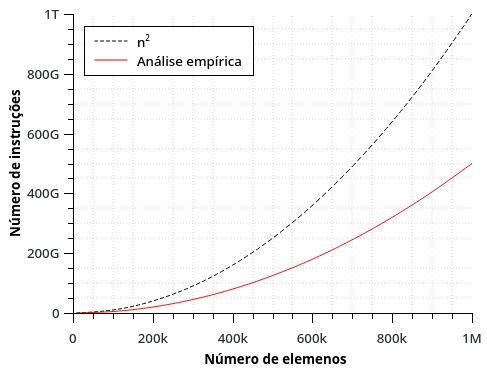
\includegraphics[scale=0.7]{images/bubble_graph.jpg}
\caption{Bubble Sort}
\label{fig:bubble}
\end{figure}

\subsection{Bubble Sort com otimizações}
Uma possível otimização para o bubble sort é atravez de uma condição de parada caso o laço interno não efetue nenhuma troca de elementos \cite{geeks:01}, quando isso ocorre significa que o vetor já está ordenado e a complexidade, para o melhor caso, passa a ser $O(n)$.

Para os casos testados, o decréscimo no número de instruções foi praticamente insignificante se comparado ao valor total. Fator facilmente observado na Figura~\ref{fig:bubble_optimized}, mostrando diferenças mínimas para o gráfico da Figura~\ref{fig:bubble}.
\begin{figure}[h]
\centering
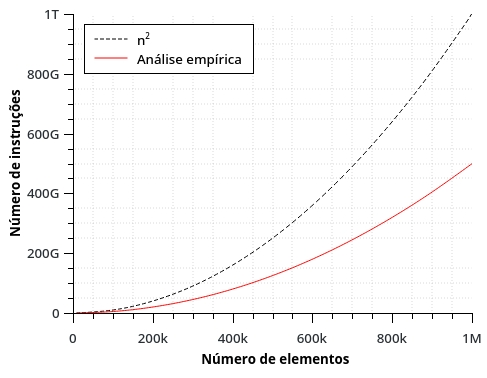
\includegraphics[scale=0.7]{images/bubble_optimized_graph.jpg}
\caption{Bubble Sort Otimizado}
\label{fig:bubble_optimized}
\end{figure}

\subsection{Insertion Sort}
A primeira iteração do algoritmo pega o segundo elemento do vetor e, se for menor que o primeiro elemento, troca-os de posição. A segunda iteração compara o terceiro elemento e o insere na posição correta de acordo com os dois primeiros elementos. Na $i^{n-ésima}$ do algoritmo, os primeiros $i$ elementos do vetor original estarão ordenados \cite{deitel:01}.

Possui complexidade $O(n^2)$ para o caso médio e o pior caso, para o melhor caso tem comportamento $\Omega(n)$. Pela análise empírica, Figura~\ref{fig:insertion}, apresentou ordem $O(nlog(n))$, pois as entradas utilizadas possuíam valores que se repetiam diversas vezes, facilitanto o algoritmo a encontrar posição correta dos elementos.

\begin{figure}[ht]
\centering
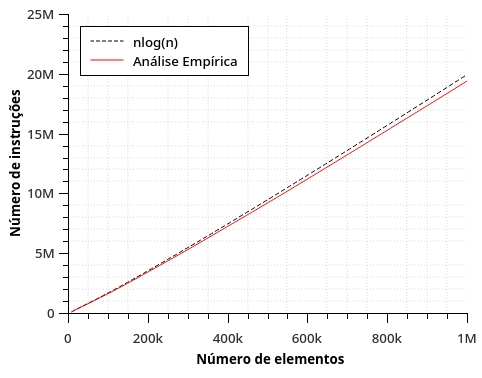
\includegraphics[scale=0.7]{images/insertion_graph.jpg}
\caption{Insertion Sort}
\label{fig:insertion}
\end{figure}
 
\subsection{Selection Sort}
A primeira iteração do algoritmo seleciona o elemento com menor valor e o troca com o primeiro elemento do vetor. A segunda iteração seleciona o segundo elemento com menor valor e o troca com o segundo elemento do vetor. O algoritmo continua até a útima iteração, onde seleciona o elemento com o segundo maior valor e o troca com o penúltimo elemento no vetor, deixando o maior valor no último elemento \cite{deitel:01}.

Possui ordem assintótica $\Theta(n^2)$ devido a laços invariantes, como pode ser observado pela análise empírica, Figura~\ref{fig:selection}.
\begin{figure}[ht]
\centering
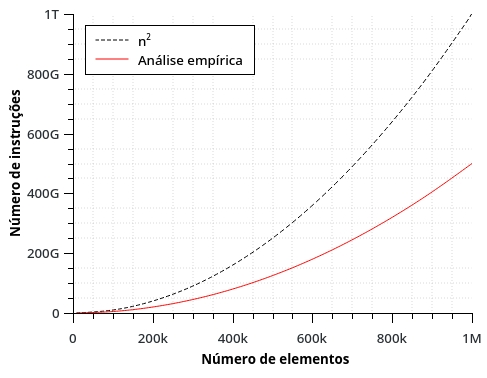
\includegraphics[scale=0.7]{images/selection_graph.jpg}
\caption{Selection Sort}
\label{fig:selection}
\end{figure}

\subsection{Merge Sort}
A ideía básica do algoritmo é ordenar um vetor dividindo-o em dois sub-vetores de mesmo tamanho até que cada sub-vetor tenha apenas um elemento, então ordena cada sub-vetor e os junta de volta, resultando em um novo vetor ordenado. Método conhecido como divisão e conquista.

Possui complexidade $\Theta(nlog(n))$ e pela análise empírica apresentou examente este comportamente, como pode ser visto na Figura~\ref{fig:merge}. 
\begin{figure}[ht]
\centering
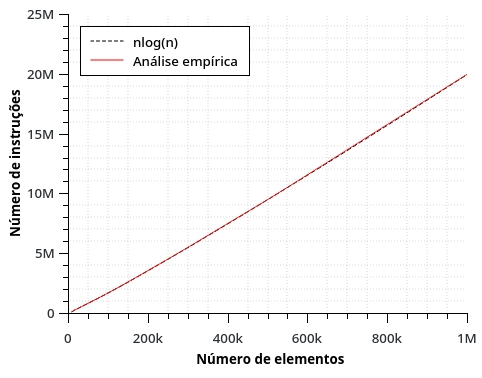
\includegraphics[scale=0.7]{images/merge_graph.jpg}
\caption{Merge Sort}
\label{fig:merge}
\end{figure}

\subsection{Heap Sort}
A idéia básica do algoritmo é transformar o vetor em uma estrutura de dados heap, a qual tem a propriedade de permitir, de forma eficiente, a obtenção e remoção dos elementos de maior valor. Repetidamente retirando o elemento de maior valor do heap e construindo o vetor ordenado do fim para o início \cite{rosetta:01}.

Possui complexidade $\Theta(nlog(n))$ para todos os casos, como também pode ser observado pela análise empírica, Figura~\ref{fig:heap}.
\begin{figure}[h]
\centering
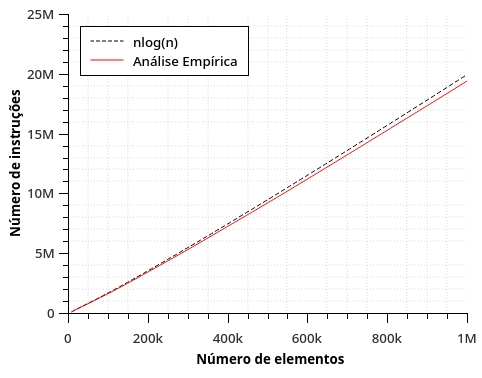
\includegraphics[width=0.7\textwidth]{images/heap_graph.jpg}
\caption{Heap Sort}
\label{fig:heap}
\end{figure}

\subsection{Quick Sort}
Assim como o Merge Sort, o Quick Sort também é um algoritmo de divisão e conquista. Ele seleciona um elemento como pivô e particiona os elementos de acordo com o valor do pivô, colocando os elementos menores a esquerda e os maiores a direita do pivô \cite{geeks:02}.

Apresenta complexidade $\Theta(nlog(n))$ para o caso médio, entretanto para o pior caso possui ordem assintótica $O(n^2)$, apesar disso, o quick sort com frequência é a melhor opção prática para a ordenação, devido aos fatores ocultos na notação $\Theta(nlog(n))$ serem bastante pequenos \cite{cormen:01}.
O principal determinante de um bom desempenho está na escolha do pivô, podendo ser:
\begin{itemize}
\item Sempre escolher o primeiro elemento como pivô.
\item Sempre escolher o último elemento como pivô. Utilizado na implementação para este trabalho.
\item Escolher um elemento aleatório como pivô.
\item Escolher o elemento do meio do vetor como pivô.
\end{itemize}

Durante a análise empírica apresentou comportamento $O(n^2)$, Figura~\ref{fig:quick}, por termos tomado o último elemento como pivô e pelo vetor a ser ordenado possuir muitos elementos de mesmo valor, tornando o particionamento ineficiente.

\begin{figure}[ht]
\centering
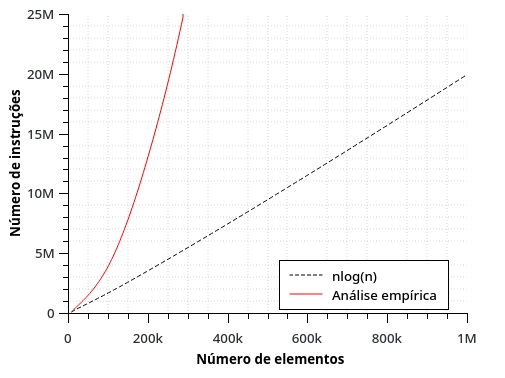
\includegraphics[width=.5\textwidth]{images/quick_graph.jpg}
\caption{Quick Sort}
\label{fig:quick}
\end{figure}

\subsection{Busca Binária}
Se nós compararmos o alvo com o elemento que está no meio de uma lista ordenada, teremos três resultados possíveis: encontramos o alvo, o alvo é menor que o elemento, ou o alvo é maior que o elemento. No primeiro e melhor caso, a busca está feita. Nos outros dois casos, sabemos que metade da lista pode ser elimida \cite{mcconnell:01}. O processo continua considerando apenas o vetor parcial onde o alvo pode estar localizado, terminando quando o vetor parcial possui apenas um elemento, ou quando o alvo é encontrado.

Sua complexidade é $O(log(n))$ e na análise empírica obtivemos exatamente isso em alguns pontos, em outros a podemos ver um comportamento constante, visto que o vetor ordenado de entrada possuia diversos entradas iguais, permitindo que o valor alvo fosse encontrado com facilidade, como pode ser observado na Figura~\ref{fig:busca}.
\begin{figure}[ht]
\centering
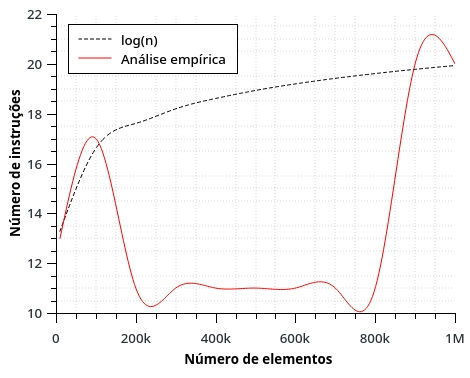
\includegraphics[width=.5\textwidth]{images/binary_graph.jpg}
\caption{Busca Binária}
\label{fig:busca}
\end{figure}

\subsection{Busca do Subvetor Máximo}
Queremos encontrar um subvetor máximo do subvetor $V[e...d]$. A divisão e conquista nos diz que devemos dividir o problema o mais igualitariamente possível, ou seja, podemos dividir ao meio, $m$, e considerar os subvetor $A[e...m]$ e $A[m + 1...d]$. Cada subvetor contíguo $A[i...j]$ em $A[e...d]$ deve estar em três lugares:
\begin{itemize}
\item inteiro no subvetor $A[e...m], e \leq i \leq j \leq m;$
\item inteiro no subvetor $A[m + 1...d], m \leq i \leq j \leq d, ou;$
\item entre $e \leq i \leq m \leq j \leq d$
\end{itemize}

Assim, o subvetor máximo $A[e...d]$ deve estar em um destes três lugares. De fato, um subvetor máximo de $A[e...d]$ deve ter a maior soma de todos os subvetor inteiramente em $A[e...m]$, inteiramente em $A[m + 1...d]$ ou cruzando $m$.

O algoritmo trabalha encontrando a maior soma do lado esquerdo do meio de $A$, $A[max-left...m]$ e a maior soma a partir do meio + 1 de $A, A[meio+1...max-right]$. Assim, o vetor máximo resultante é entre $A[max-left...max-right]$ \cite{foleiss:01}.

Apresenta complexidade $\Theta(nlog(n))$ e foi examente o que obtivemos através da análise empírica, como pode ser visto na Figura~\ref{fig:subvetor}.
\begin{figure}[ht]
\centering
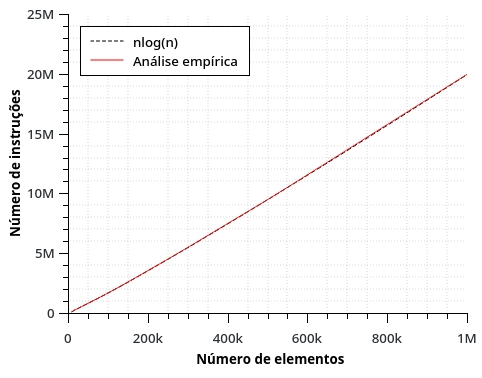
\includegraphics[width=.5\textwidth]{images/subvetor_graph.jpg}
\caption{Busca do Subvetor Máximo}
\label{fig:subvetor}
\end{figure}

%%% Local Variables:
%%% mode: latex
%%% TeX-master: "Artigo"
%%% TeX-command-extra-options: "-shell-escape"
%%% End:
